\documentclass[../Article_Model_Parameters.tex]{subfiles}
\graphicspath{{\subfix{../Figures/}}}
\begin{document}
	
	\section{General function approximators} \label{CH: RBF}
	
	\subsection{Radial Basis Function}
	
	An alternative approach to the first principle modelling of physical process is to apply general function approximators and train them based on a dataset. Such an approach has an advantage of not pre-assuming a structure of a model, which results in higher flexibility of a model. On the other hand, this come with a cost of higher number of parameters to be fitted and choosing appropriate function approximator. In this work, a Radial Basis Function (RBF) is used to define $\frac{dc_s}{dt}$ based on a dataset. RBF is a sum real-valued functions (so called kernels) $\delta$ whose value depends only on the distance between the input and some fixed point, called a center $c$, so that $\delta(x) = \delta(||x-c||)$. The distance is usually Euclidean distance, although other metrics are sometimes used. Sums of radial basis functions are typically used to approximate given functions $y(x) = \sum_{i=1}^{N} w_i \delta(||x-c_i||) + b$. Where $N$ corresponds to the number of kernels, $w$ to weight in the summation and $b$ is a bias. The kernel can be defined as a Gaussian, Inverse quadratic, Inverse multi-quadratic, Polyharmonic spline etc. In this work, the two-dimensional Gaussian is used. All the kernels are assumed to have the same shape, which means the all have the same widths in the same direction.
	Following observation from {\color{red}article 1}, the two independent variables are normalized concentration of the solute in the solid phase, defined as $\tilde{c}_s(t) = 1 - \left(\frac{c_s(t)}{c_{s0}}\right)$, and the Reynolds number.
	
	{\footnotesize
		\begin{align} %
			\frac{dc_s}{dt} &= \sum_{i=1}^{N} w_i \delta(||x-c_i||) + b \\ \nonumber
			&= \sum_{i=1}^{N} w_i \exp \left( - \frac{ \left( \tilde{c}_s(t)-\tilde{c}_{si}^c \right)^2 }{2\sigma_1^2} - \frac{ \left( Re(t)-Re_i^c \right)^2 }{2\sigma_2^2} \right) + b \label{EQ: RBF}
		\end{align}
	}
	
	where $\tilde{c}_{si}^c$ and $Re_i^c$ correspond to centrers of each Gaussian kernels as defined above. $\sigma_1$ na $\sigma_2$ corresponds to the width of each kernel in direction of $\bar{c}_{si}$ and $Re_i$, respectively. The unknowns of this equation are $N$, $w_i$, $\tilde{c}_{si}^c$ and $Re_i^c$. If $N$ is pre-selected, then the total number of unknowns can calculated as $3N+3$. The new process model is defined by substituting Equation \ref{Model_solid} with \ref{EQ: RBF}. The parameter estimation procedure follows {\color{red}article 1}. The obtained parameters are presented in Table \ref{table:RBF}.
	
	\begin{table}[H]
		\centering
		\adjustbox{max width=\textwidth}{%
		\begin{tabular}{l|ccccccc}
			i				&  	1		&  2&  3& 4& 5& 6&  \\ \hline
		$\tilde{c}_{si}^c$ 	&   -0.294	&  1.465&  -0.303&  1.124& -0.025& -0.424& \\
		$Re_i^c$			&   0.410&  0.281&  0.057&  0.913& 1.185& 0.269& \\
		$w_i$				&   2.001&  0.541&  6.569&  -1.208& -0.663& 6.123& \\
		$\sigma_1^2$		&   0.433&  &  &  & & & \\
		$\sigma_1^2$		&   0.051&  &  &  & & & \\
		$b$					&   -0.131&  &  &  & & &
		\end{tabular} }
		\caption{Parameters of the RBF}
		\label{table:RBF}
	\end{table}
	
	Good agreement between the simulation results and the dataset can be observed, as presented by calculated mean square error and standard deviation as presented in Table \ref{tab:Modelling_Error}.
	
	\begin{table*}[h]
		\centering
		\adjustbox{max width=0.9\textwidth}{%
			%\small{
				\begin{tabular}{ l|ccccccccccccc }
					\hline 
					Experiment			&1 		& 2 		& 3 	 & 4 	  & 5 	   &6 	   & 7	   & 8	   & 9	   & 10    & 11    & 12	\\  \hline
					Mean squared error	&0.0049 & 0.0100 	& 0.0042 & 0.1255 & 0.0401 &0.0368 & 0.0061& 0.1292& 0.0084& 0.0109& 0.0028& 0.0130	\\  
					Standard deviation of error	&0.0705 & 0.0619 	& 0.0334 & 0.1422 & 0.0791 &0.0704 & 0.0779& 0.1313& 0.0466& 0.1069& 0.0287& 0.0477	\\  \hline
			\end{tabular} }
			\caption{Error between experimental data and model predictions}
			\label{tab:Modelling_Error}
		\end{table*}
	
	\begin{figure}
		\centering
		\begin{subfigure}[b]{0.45\columnwidth}
			\centering
			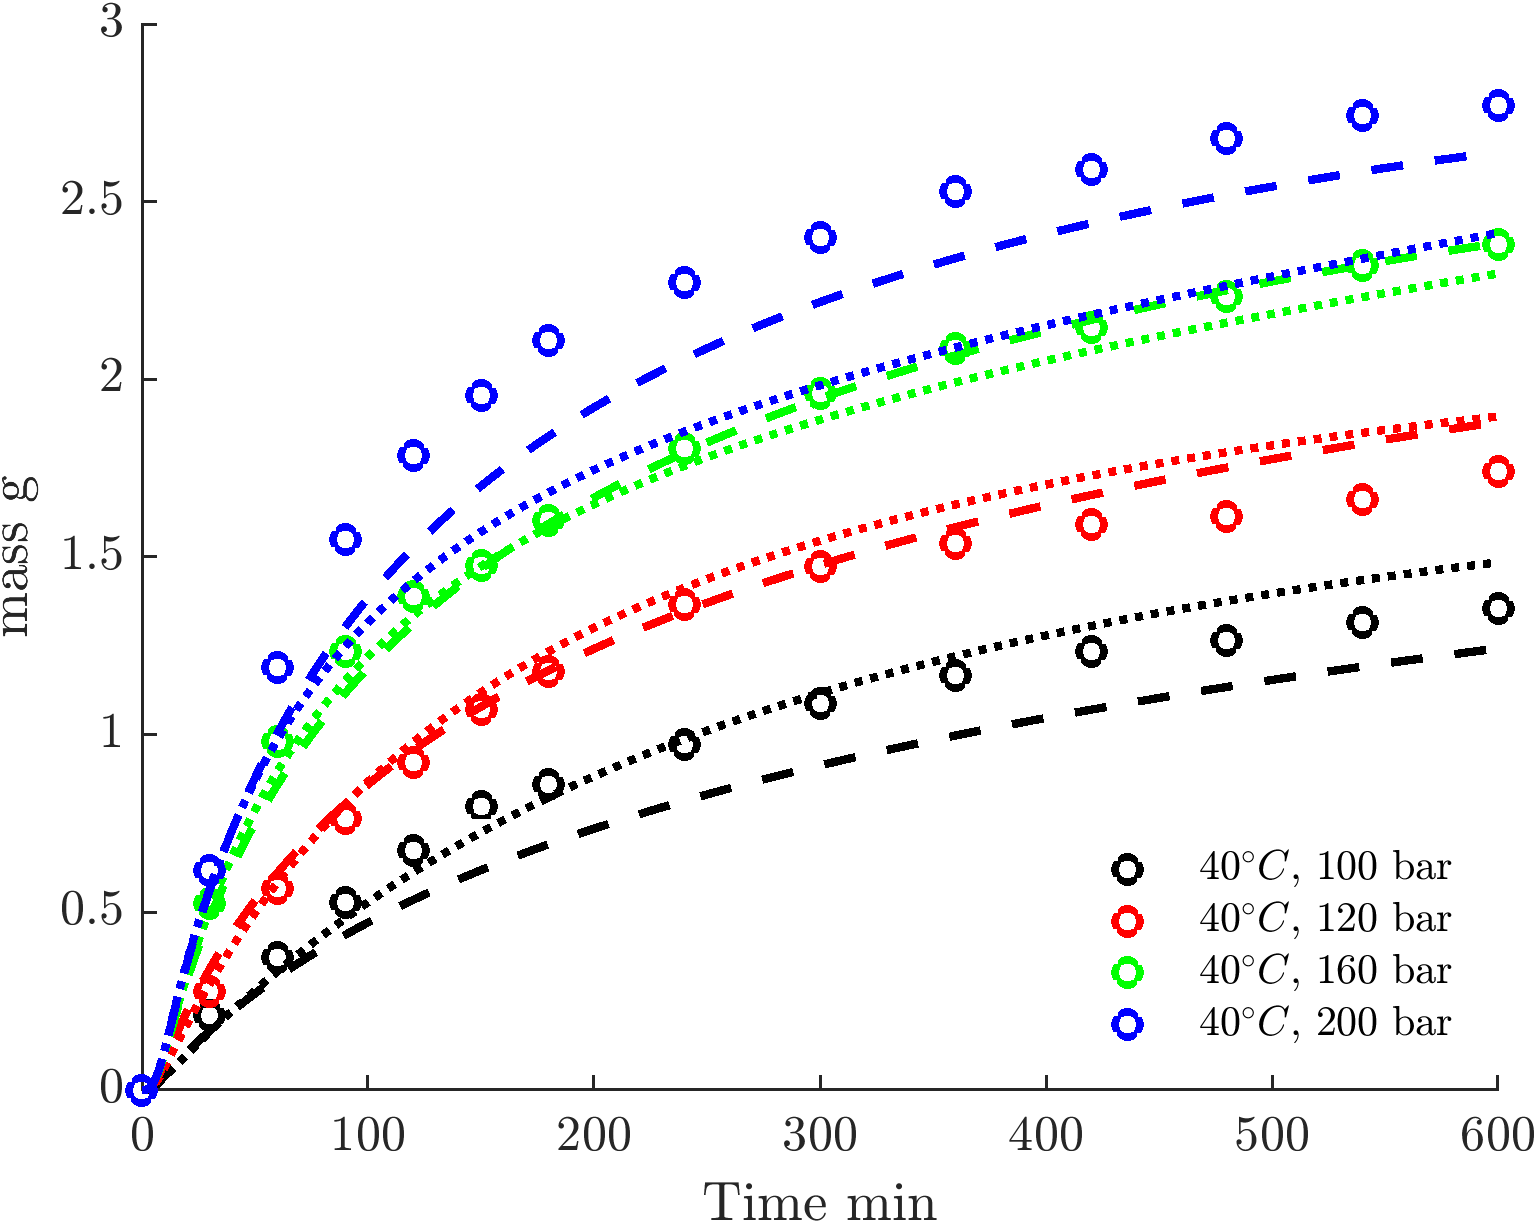
\includegraphics[width=0.95\columnwidth]{/Results/RBF_1.png}
			\caption{Simulation results at $6.67\cdot 10^{-5}$ kg/s}
			\label{fig:RBF_1}
		\end{subfigure}
		\hfill
		\begin{subfigure}[b]{0.45\columnwidth}
			\centering
			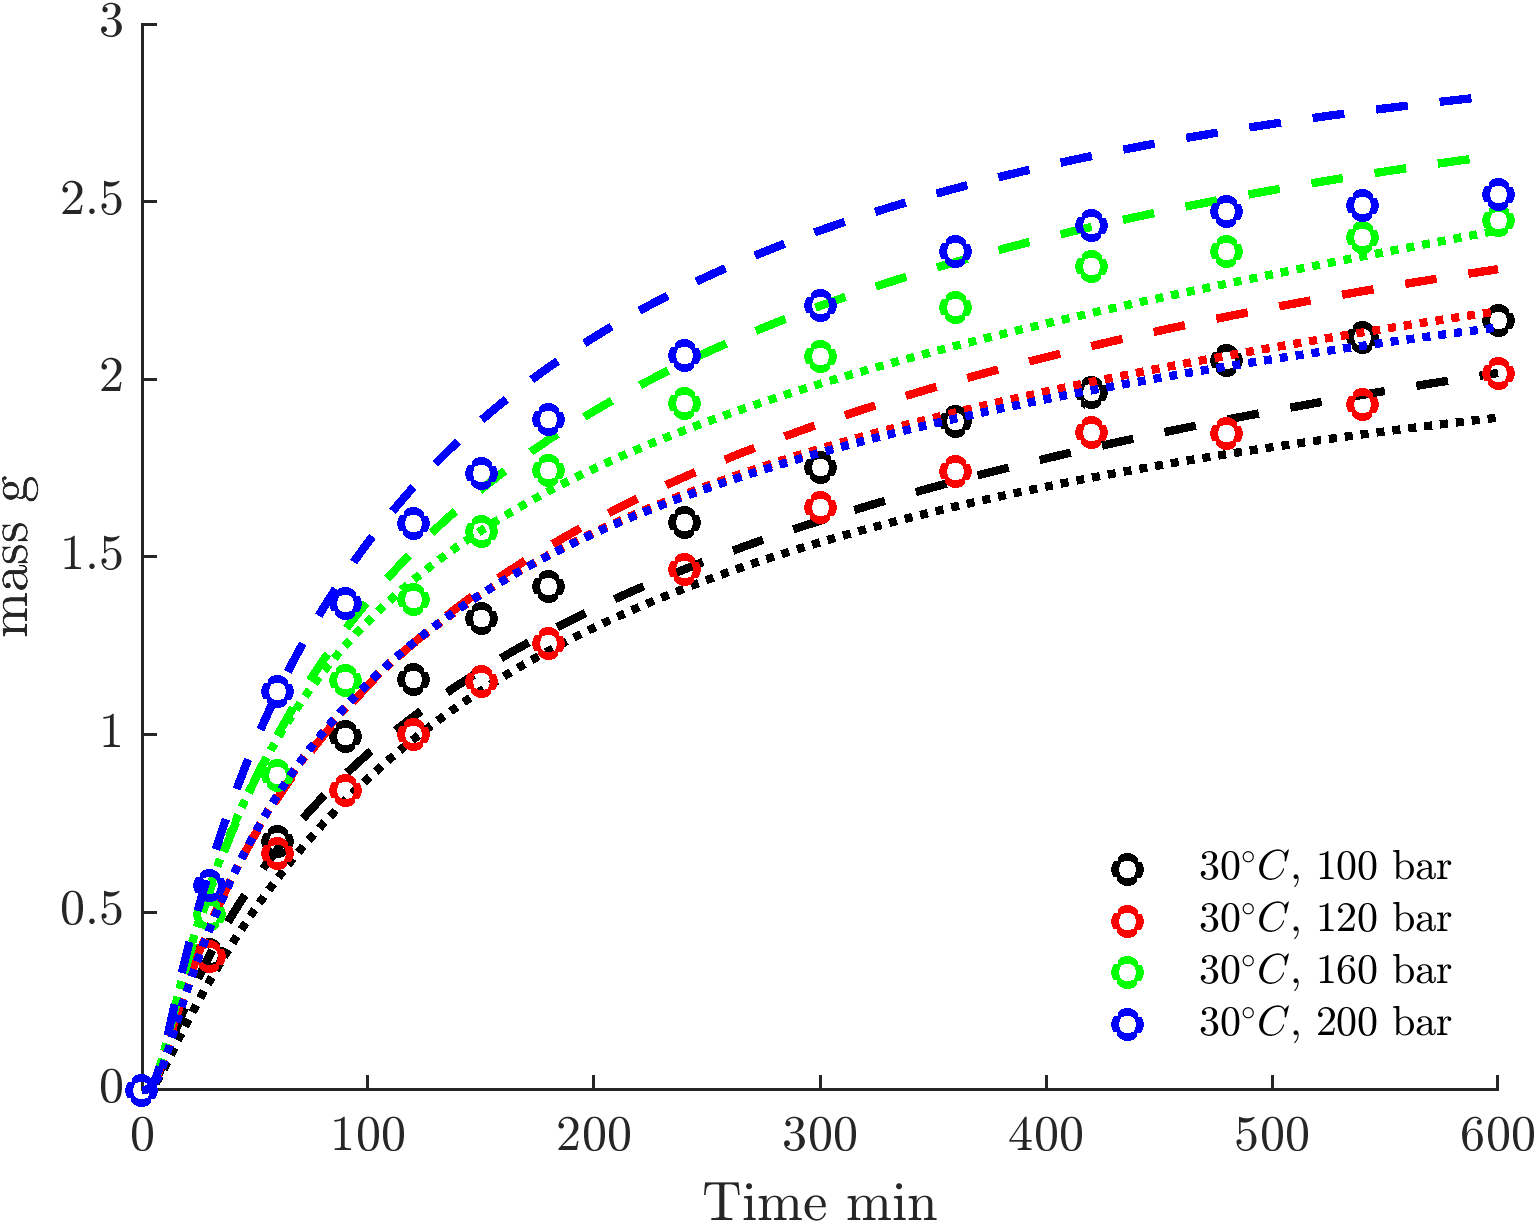
\includegraphics[width=0.95\columnwidth]{/Results/RBF_2.png}
			\caption{Simulation results at $6.67\cdot 10^{-5}$ kg/s}
			\label{fig:RBF_2}
		\end{subfigure}
		\hfill
		\begin{subfigure}[b]{0.45\columnwidth}
			\centering
			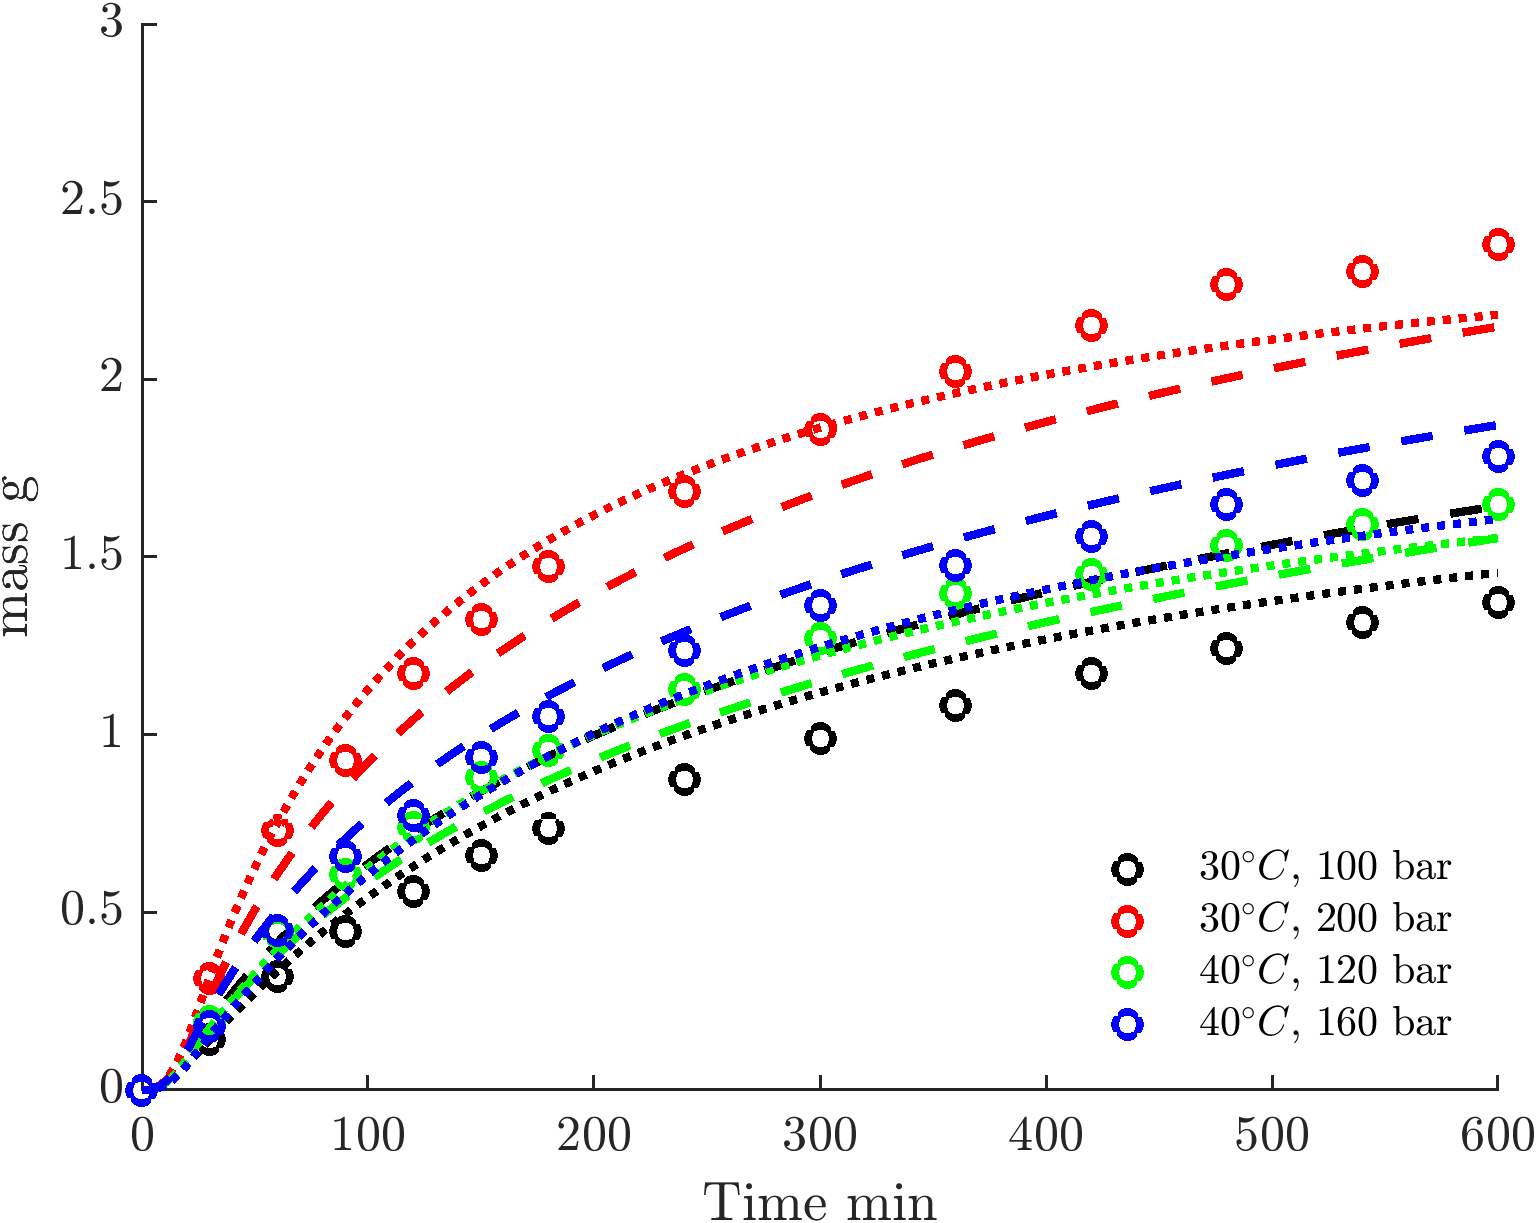
\includegraphics[width=0.95\columnwidth]{/Results/RBF_3.png}
			\caption{Simulation results at $3.33\cdot 10^{-5}$ kg/s}
			\label{fig:RBF_3}
		\end{subfigure}
		\caption{Comparison of models against the dataset}
		\label{fig:three graphs}
	\end{figure}
				
\end{document}